\icode[magenta]{E-MD-SI-L4-261111-001}
如图所示，\(A\)、\(B\)、\(C\)三个物体的质量分别为\(2m\)、\(2m\)、\(3m\)，其中物体\(B\)和\(C\)通过轻绳连在一起，物体\(A\)和\(B\)通过跨过光滑定滑轮的轻绳连在一起，物体\(A\)与轻弹簧上端连在一起，轻弹簧下端固定在地面上，初始时三个物体均保持静止(重力加速度为\(g\))。下列说法正确的是\paren[]
		
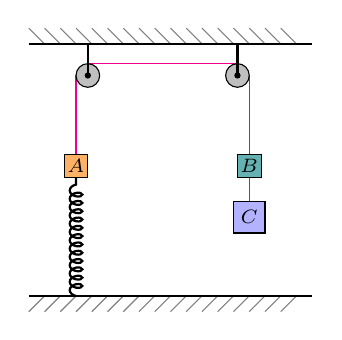
\begin{tikzpicture}[font=\scriptsize]
	\draw[thick,decoration={aspect=.6,segment length=3,amplitude=.8mm,coil},decorate] (0,0)--(0,1.5);
	\draw[magenta] (0,1.8)--(0,2.8) (.15,2.95)--(2.05,2.95) (2.2,2.8)--(2.2,1.2);
    \draw[fill=gray!50] (.15,2.8) circle(.15) (2.05,2.8) circle(.15);
    \draw[thick] (.15,2.8)--(.15,3.2) (2.05,2.8)--(2.05,3.2);
    \fill (.15,2.8) circle(.04) (2.05,2.8) circle(.04);
	\draw[fill=orange!60] (-.15,1.5) rectangle(.15,1.8)node[midway]{\(A\)};
    \draw[fill=teal!60] (2.05,1.5) rectangle(2.35,1.8)node[midway]{\(B\)};
    \draw[fill=blue!30] (2,.8) rectangle(2.4,1.2)node[midway]{\(C\)};  
	\foreach \x in {-.6,-.4,...,2.8}{
		\draw[gray] (\x,-.2)--++(.2,.2);
		\draw[gray] (\x,3.4)--++(.2,-.2);}
	\draw[thick] (-.6,0)--(3,0) (-.6,3.2)--(3,3.2);
\end{tikzpicture}
\begin{choices}
	\item 初始时弹簧处于压缩状态
	\item 剪断\(A\)、\(B\)间轻绳后瞬间物体\(B\)、\(C\)间轻绳拉力为\(3mg\)
	\item 剪断\(B\)、\(C\)间轻绳后瞬间物体\(A\)的加速度为\(\frac{g}{2}\)
	\item 剪断\(B\)、\(C\)间轻绳后瞬间物体\(A\)、\(B\)间轻绳拉力为\(\frac{7mg}{2}\)
\end{choices}
\begin{answer}
    D\qquad 提示：
\end{answer}